\chapter{A prototypical implementation for a source-to-source transformation tool generating cache friendly code / COOP}\label{prototype}
We have the tools, to programmatically strip down a program's records and reassemble it in a fashion that suits our needs (Clang). So it is time to consolidate our goals for a prototype. First of all, it should be fairly easy to integrate the tool into a working environment/existing tool-chains. For reasons mentioned in \refsec{motivation} we can not ever expect our tool to be used otherwise. As simple as that sounds this leads to interesting design choices, we will briefly discuss in \refsec{stand_alone_tool}.\\
Even though the tool's scope will be limited due to being a one-man project it should demonstrate, that automated OOP to DoD data layout transformations are possible. To do so we will try to implement a Hot/Cold Split \refsecp{hot_cold_splitting}. Instead of completely changing the program's data layout this way we can implement a data driven optimization, that seems to be relatively easy to perform automatically. We will see that while hot/cold splits are conceptually trivial, performing a particular split is only beneficial given the meta information about the data is correct. Automating the retrieval of such meta data will be a fundamental mile-stone in development and set the base for all further source transformations \refsecp{data_aggregation}.\\
Ideally we desire that the target program should provide zero additional programming overhead to our tool, so the process of transforming the target program into a cache friendly pendant will not interfere with the process of solving the problem. We will later see why this entails massive additional responsibility for our tool \refsecp{auto_oop_to_dod}.\\
The tool needs to maintain the semantic integrity of the original source code. Even though changing the programs data layout will definitely affect the data access patterns (thus will actually change the programs data flow) the result must not be distinguishable from the original in other terms than performance. \Refsec{deep_copy_emulation} will show why this prerequisite will yet rely on additional effort.\\
We want the resulting program to be faster, measuring frame-times as well as cache-misses. However optimizing the data layout of a program will only really affect software, that heavily relies on it. For example transformations on multidimensional arrays are perfect candidates for locality optimizations \mcp{bryant}{617}. While it is difficult to guarantee performance boosts for every possible source program we should rather aim for: Improves most programs. It definitely must not make the program slower though! 
\newpage
\subsubsection{Summarized Goals}
\begin{itemize}
	\item Easily integrable in existing working environment
	\item Automated OOP to DoD data layout/access transformation
	\item Zero additional programming overhead for the user
	\item Improve most programs; mustn't worsen them.
	\item Maintain semantic integrity

\end{itemize}
From this point on we will talk about the specifics of the prototypical implementation called COOP (\textbf{C}ache friendly \textbf{O}bject \textbf{O}riented \textbf{P}rogramming) and will refer to the tool by this name.

\section{Stand Alone Tool}\label{stand_alone_tool}
Even though COOP is not aimed to be a commercially used tool, thinking of how such a technology could reach the industry it becomes clear, that the less COOP implicates structural changes to the build setup or an engine's tool-chain the higher are its chances of being used. Hence even though we use the Clang front end infrastructure to implement our solution, we do not want potential users of COOP to depend on LLVM/Clang. Therefore we first need to find a way to implement our solution utilizing LLVM/Clang in the right way.\\ 
There are various ways to use the framework LLVM/Clang provides. Since we are trying to improve a target programs performance by alternating parts of it, the classification of our tool fits is a \textit{Code Optimization} \mcp{aho}{583}. Compilers usually carry out optimization-passes either on the IR they provide or on the generated code in a machine specific way \reffigp{compiler_phases}. While LLVM already comes with numerous optimization passes that are either \textit{Analysis Passes}, \textit{Transform Passes} or \textit{Utility Passes}, it provides a framework to implement and register custom passes as well. However implementing an LLVM pass binds the user to the LLVM/Clang tool-chain \mc{llvm_passes}. Optimization passes are not interchangeable between independent compilers and if possible we should avoid expecting users to change their build setup for us.\\\\
The Clang front end functionality provides infrastructure to access syntactic and semantic information about programs. A so called \textit{Clang tool} can be created in three different ways.
\textit{LibClang} is a high level interface to clang. It already provides AST traversal yet does not give us full control over it. \textit{Clang Plugins} provide full control over the AST as part of compilation. They are dynamically loaded by the compiler and can make or brake a build. However this again ties us to the LLVM tool-chain. Finally \textit{LibTooling} is a C++ interface aimed at writing stand alone tools. It also provides full control over the AST is however subject to change and maintaining a tool based on it means continuous adaptation to new versions. \mc{clang_tools}\\
When providing a stand alone tool, any build setup can adapt easily to it by invoking it manually. For example a \textit{Makefile} could easily use COOP either before compilation or for a target of its own (e.g. make coop).\\
The Clang front end functionality alone will limit us to source-to-source transformations, meaning in terms of compilers our target language equals our source language. This is rather uncommon, since an optimization is usually realized as a pass that works on intermediate representations or machine code and will not ever affect the source code we see in our IDEs. However an advantage of this approach is, that when the result of our tool is C++ source code, the whole bandwidth of optimizations provided by the compiler already can still be applied in a manner the compiler expects to do. We can not rely on the compiler to optimize our custom optimization pass. Also this way the optimized code remains relocatable.\\\\
But there is one major disadvantage in this approach. A pre-compile- or 'source-to-source' optimization pass implies sudden structural changes to the code base. So the issue of 'losing the desired abstraction level' would just be postponed. This is irrelevant as long as the optimization is applied only before a shipping build is generated, but integrating COOP into an agile development process would only work with the help of version control systems, so its changes can be undone easily and abstraction is only ever lost, when intended and reversible.\\
Speaking of agile development or any development model relying on short iterations a tool like COOP would only make sense when it's fast. As we will see later on, traversing numerous ASTs for a complete code base gets slow really (really) fast \refsecp{build_times}.\\\\
Since COOP will work on source files rather than on binaries we will need to present it the files, that it is supposed to work on. There is of course always the option of manual forwarding per command line, but in favor of simplicity for example a compilation database can be generated automatically by some build tools and is therefore a convenient bearer of this information. For example when using CMAKE one can simply add '\textit{set(CMAKE\_EXPORT\_COMPILE\_COMMANDS ON)}' to the \textit{CMakeLists.txt} file to create a \textit{compile\_commands.json} compilation database.\\
Another advantage of a compilation database is less manual overhead on COOPs integration. Files that include certain other files (like H/HPP-files) will not be processable if no information is given on where to find the included files. The tool instance, that is worked with to access Clang's functionality is in the end a proper compiler front-end that will go through each of the aforementioned steps of Lexing and Parsing and a complete set of symbols is imperative for a compiler to work.\\
In the end providing files manually will work, but will come with significantly more effort, so offering the option of providing a compilation database can accommodate the user to great amounts.

\section{Automated split-candidate evaluation through static analysis}\label{auto_oop_to_dod}
Splitting a record's hot-/cold fields is in essence a trivial transformation when done manually and when given the set of hot/cold fields. Create a struct; move cold fields in it; create a pointer to a cold-struct instance in original record; Change all accesses to cold fields to accesses on cold-struct field pendants, respectively. This is why the Hot/Cold Split was deemed a fitting exemplary for a prototypical proof-of-concept implementation. To do so, first of all we need the right AST nodes.\\
Comfortable access on the records and their fields is granted by appropriate AST matchers. After creating a source file's AST we can easily match against any record declaration in it and the moment we have a \textit{CXXRecordDeclaration} node we have access to numerous helpful methods, that give us it's fields, constructors, methods, base classes etc. COOP defines a handful of matchers and callback-routines that filter wanted data (see Code \ref{matchers} line 1 to 6).
\begin{lstlisting}[language=C++,name={Some matchers used by COOP to filter relevant AST nodes and their utilization },label={matchers}]
auto file_match =
	isExpansionInFileMatching(coop::match::get_file_regex());
DeclarationMatcher records =
	cxxRecordDecl(file_match, unless(anyOf(isUnion(), isImplicit())).bind("record_binding");
StatementMatcher members_used_in_functions =
	memberExpr(file_match, hasAncestor(functionDecl(isDefinition())));

MatchFinder::MatchCallback *callback = new MemberRegistrationCallback();

MatchFinder data_aggregation;
data_aggregation.addMatcher(records, callback);

data_aggregation.matchAST(ASTs[0]->getASTContext());
\end{lstlisting}
The \textit{file\_match} matcher for example makes sure, we are not operating on - let alone transforming - files, that do not originally belong to our project, like system headers. The \textit{records} matcher will give us all the records found in the compilation unit \textit{unless} it is a union or an implicit match \refsecp{a_usfl_int}. By binding a matcher to a string we can retrieve the matcher's result in a callback routine. The callback needs to be implemented as a class definition extending Clang's own \textit{MatchCallback} \refcodep{member_registration_callback}. Callbacks can then be added to a \textit{MatchFinder} instance and finally be applied to an AST (see Code \ref{matchers} line 8 to 13). The \textit{MemberRegistrationCallback}'s overridden run method accesses the result's nodes through the string association we gave it earlier. COOP now registers the record's fields by remembering the pointers to their AST nodes. This way we will have access to the nodes' contexts at any time.\\\\
\begin{lstlisting}[language=C++,name={Callback definition to register the records' members}, label={member_registration_callback}]
class MemberRegistrationCallback : public MatchFinder::MatchCallback {
public:
	std::map<const CXXRecordDecl*, std::set<const FieldDecl*>> class_fields_map;
private:
	void run(const MatchFinder::MatchResult &result)override{
		const CXXRecordDecl *rd = result.Nodes.getNodeAs<CXXRecordDecl>("record_binding");
		for(auto f : rd->fields()){		
			class_fields_map[rd].insert(f);
		}
	}
};
\end{lstlisting}
Unfortunately even though collecting the relevant parts of our target program is fairly simple, the semantic understanding of the compiler about our fields is very limited. Even though Clang offers a vast set of methods to gather information about a record/field there is no such thing as a '\textit{bool isFieldHot(const clang::FieldDecl* fd)}' function. The requirement for zero additional programming effort challenges COOP to endeavor in static analysis.

\subsection{Data aggregation}\label{data_aggregation}
One of the most challenging tasks for COOP is to identify a record's fields as hot or cold. Since we do not want to rely on the programmer to give that information to us (or even for him/her to figure it out) we need to check whether or not a field is used frequently. We need to know where, how often and with which other fields of the same record it is used.\\
As a centralized point of reference COOP will construct a \textit{will not} instance for each record, that will hold references to all the AST nodes that are relevant to us. Besides a record's fields, the \textit{will not} instance will know about all the functions that use its fields and all the loops that use its fields. It is not enough to rely on the CXXRecordDecl AST node, since it will not be able to tell us where it's instances are used. For now it will function as a mere cache to our ASTs to quickly access a record's important nodes, that can be distributed all over our code base and thus be distributed among different ASTs.\\
To collect the data about how/where our records are utilized, we define a several AST Matchers and callback routines, for example:
\begin{itemize}
	\item MemberRegistrationCallback $\rightarrow$ registers records and their fields
	\item FunctionRegistrationCallback $\rightarrow$ registers functions and their member expressions
	\item LoopMemberUsageCallback $\rightarrow$ registers loops and their member expressions
\end{itemize}
After all the compilation units have been transformed into ASTs, the functions and loops need to crosscheck all the records, to see if they are relevant to any of them. If they work with a records fields, they are remembered by the respective \textit{will not}. This way we can generate a matrix that encodes field-function/field-loop information in numerical values, an important step towards being able to evaluate and prioritize those relationships in a generic way.
\begin{figure}[!htbp]
	\centering
	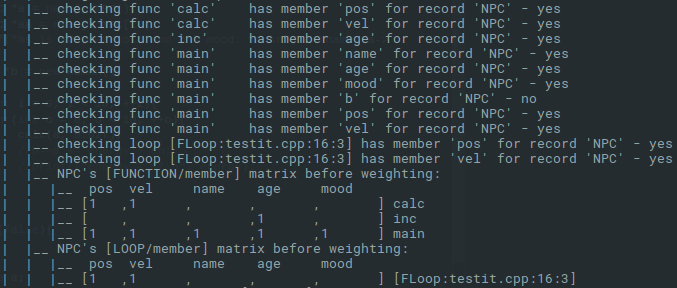
\includegraphics[width=.7\linewidth, height=0.3\linewidth]{PICs/npc_crosscheck_matrix}
	\caption{Excerpt of coops output on exemplary NPC and some arbitrary functions/loops}\label{npc_crosscheck_matrix}
\end{figure}
Ultimately our evaluation faces a problem, that scales with our implementation details. Similarly to how we evaluated cache-line utilization in \refsec{soa} for each function we could determine (estimate) its behavior for a certain Hot/Cold split in a brute force kind of way. So we can make statements about which split would be the best.\\
Through a function/member matrix we can determine cache utilization for each function individually. The number associated with a member expression can be interpreted as 'how much punishment would it mean to externalize me for this function'. For a simple case like \reffig{npc_crosscheck_matrix} we could easily determine, that the function \textit{calc} would like to have the \textit{name, age, mood} field subset externalized. But externalizing either \textit{pos} or \textit{vel} would mean loading the respective cold struct instance as many times, as it's associated value. The \textit{punishment} specifically would depend on how big the cold struct instance is, which also varies depending on whether or not each other field is hot or cold.\\
More formally there are $\sum_{k=0}^{n} \frac{n!}{k!(n-k)!}$ different combinations of how a record can be split, where $n$ is the number of fields in the record and $k$ is the number of fields to hive off. As an example we could imagine a record with 10 fields. Conclusively there are 1023 different combinations of possible splits. Checking each function let's say 50 would result in $> 50.000$ computations. Since we specifically regard the loops as well this number will become even higher - per record - and eventually with actual big code bases shoot through the roof.\\
So instead of cross checking each split scenario with each function/loop we would like to consolidate each fields 'importance' or it's 'weight' in a centralized spot, that will be checked against $n-1$ other fields instead.

\subsection{Metric for evaluation of field usages}\label{metrics}
We described fields to have relations to loops/functions. Expressing these relations numerically might get us into regarding existing metrics, hoping they provide information we can process. The values assigned to a relation could be based on a lot of things, so at this point we should contemplate on what would be the most useful piece of information. Even though we will see, that the chosen metrics do not suffice our needs perfectly, they have aspects and methodology we can utilize for our purpose.
\subsubsection{Cohesion metrics}
An automated Hot/Cold Split will eventually externalize a subset of fields into another record. We do so by finding the hot data and conversely the cold data \refsecp{hot_cold_splitting}. When thinking about why the cold data was put together with the hot data in the first place we remember, that it might be due to our unfortunate abstraction \refsecp{oop_bad_abstraction}. Talking about splitting records on account of their fields' relations sounds like what \textit{cohesion metrics} try to solve.\\
Cohesion in a module describes to what extend, that module serves a single logical task \mcp{ingeno_cohesion}{172}. Its purpose is to indicate on how well a software architecture is defined. Modules with good cohesion have proven to be reusable and easy to maintain, whereas low cohesion indicates, that changes in the code will affect other parts of the code resulting in increased effort in development as well as in testing \mcp{ingeno_cohesion}{172}.\\
There are several types of cohesion, that are used to classify a module, like \textit{Coincidental Cohesion}, where elements are grouped with no logic concept for example in a utility or helper collection. This is considered to be low cohesion and should be avoided.\\
\textit{Logical Cohesion} describes what we have found to be bad abstraction patterns coming with OOP. We group logically related elements, because they share a context. Consequently we will collect lots of fields, that belong to different domains. Cohesion metrics also recommend to avoid this kind of design.\\
\textit{Temporal/Procedural Cohesion} both describe a grouping of fields, because they are processed at the same time/in a certain order. So basically when they share temporal locality. Even though we discussed earlier \refsecp{cpucu} that trying to design around principles of locality is one of our main goals in DoD, thinking in an OOP way this is rather bad, because it might promote monolithic class- and method definitions. Again cohesion metrics want our record definitions to follow a single task. This level of cohesion is considered to be acceptable but not ideal \mcp{ingeno_cohesion}{174}. But DoD does not argue here actually. Temporal/Procedural cohesion think in a bigger scale than what we meant earlier with temporal locality. For example grouping independent elements because they all are related to system startup/cleanup even though they do not interact.\\
This is another example of where we find a big gap between OOP and DoD at first glance but they actually conform with each other for the most part, only differing in motivation.\\
Working our way up to the notion of an \textit{ideally} cohesive model, we pass a few other levels until we reach \textit{Functional Cohesion}. This level describes a module to group elements sharing a domain. The module will therefore serve a single purpose and changes to it will not affect code of other domains. Note that OOP very well allows for good abstraction, but again the inherent problem we face is that our intuitive abstractions do not accommodate neither software design nor our hardware. More importantly this definition of 'desirable cohesion' fits our needs to implement a Hot/Cold split, so cohesion metrics might bear the right tools, to accommodate us.\\\\
There are a hand full of metrics like \textit{LCC} (Loose Class Cohesion)  and  \textit{TCC}  (Tight  Class  Cohesion)\mcp{tcclcc}{3} or the probably well known \textit{LCOM} (Lack of Cohesion in Methods) \mcp{cohesion}{25}. Since cohesion metrics operate on object oriented code, they usually work with methods, as groups of field subsets. For example the LCOM defines a module's cohesiveness to be the "\textit{number of pairs of methods operating on disjoint sets of instance variables, reduced by the number of method pairs acting on at least one shared instance variable}"\mcp{lcom}{8}.\\
While cohesion metrics have a striking similarity in their procedure (splitting records according to their field usages), unfortunately they do differ in their intention and result. As for our Hot/Cold split, we intend to be a performance optimization and are ready to group any fields, that share spatial/temporal locality. Ultimately our Hot/Cold Split will usually automatically divide a record into domain specific sub sets, its focus however is to minimize a record's stride for cache utilization. This means we could easily end up externalizing a domain related field for the sake of faster computation.\\\\
But all is not lost, because cohesion metrics provide us with proven methodology to identify and evaluate relations in a module (record) in numbers we can compare. We also learned, that to better fit our purpose, a target metric should regard our code's performance and/or size (memory stride). 

\subsubsection{Asymptotic Notations}\label{asymptotic_notations}
An asymptotic notation or more famously O-notations describe an algorithm's complexity \mcp{onotation}{44}. It is not a measurement tool to actually evaluate the performance or memory size an algorithm uses since these depend on hardware/architecture/compilers. It describes how an algorithm scales depending on the problem size and defines upper-/lower borders for it's (asymptotic) growth depending on which notation is used. Hence the name because it deals with the \textit{order} of an algorithm.
There is for example the $\Theta$-notation that expresses asymptotic upper- and lower bounds for a given procedure.
Specifically the Big O-notation (or Landau's symbol) describes the worst-case for a procedure (asymptotic upper bound). Dealing with bounds makes sense because depending on the input (problem size), performance as well as needed memory space might vary drastically. Using the O-notation we can get estimations about a functions running time only by looking at its overall structure \mcp{onotation}{47}\\
An actual static performance analysis of code would break down the instructions to those we can find in the hardware's instruction set (depends also on the compiler), to get a grasp of how many cycles they need and ultimately how a cycle translates to (probably) nanoseconds.\\
The O-notation in its essence will also look at the instructions a procedure makes, when looking at the code. However it builds terms by evaluating control flow statements and eventually will omit constants and all but the highest order term. Expressed as a polynomial $g(n) = 5n^2+3n$ would translate to $g(n) = O(n^2)$. Since $g(n)$ is of order $n^2$ the equals notation is not perfectly correct but commonly used. Leaving out constants and low order terms is due to their insignificance considering large $n$. After all it describes asymptotic behavior.\\
In the best case a procedure is of order $O(1)$, which means no matter how big the problem becomes it will not affect our performance further. This is the case for each procedure, that operates on a fixed amount of parameters (for example typical getters/setters). While even a setter can consist of several instructions, let's say for example 3, it would translate to $3\cdot O(1)$. After omitting the constant $3$ we are left with $O(1)$. It is referred to as \textit{constant} growth.\\
Loops oftentimes iterate over dynamic ranges, so when a loop is operating instructions $n$ times it is denoted as $O(n)$ or has \textit{linear} growth.\\
Nested loops are often denoted as $O(N\cdot M)$, where N and M represent the iterations for the outer- and inner loop. In cases where N and M are equal we refer to it as \textit{exponential} growth or $O(n^2)$.\\\\
For our use case classifying our functions like this could be useful. After identifying the relevant functions (those that use our records' fields), we could evaluate them by determining their order. We could see which functions are the 'slowest' and thus reduce memory stride on the records they utilize. This could work by simply defining each field, that is used in those functions as hot. Functions that are known, to be slow, could now operate on hot data exclusively.\\\\
Unfortunately this bears some problems. A high ordered function might interact with our records very briefly (or not at all), yet would be considered a criteria for deciding which fields are hot/cold. This alone illustrates why we can not blindly apply asymptotic bounds as a criteria. We have to adapt it to our motivation, by only considering or prioritizing instructions, that are (or imply) field usages, yet again only considering our fields might falsify a denotation of the function.\\
There often will not be the one slow function, the \textit{single point of bottleneck}. Identifying a functions members as hot, in order to speed up that function might work, but might just as well worsen each other remaining function. Whether or not a field is to be considered hot has to be determined individually with their groupings (uses in functions) as a relevant indicator rather than a decisive factor.\\
Omitting constants and low order terms might provide fair estimations for large $n$, but not every program operates on huge amounts of data. Of course software, that does not depend on its data layout very much probably will not significantly benefit from a Hot/Cold split, but lower order parts of a procedure might affect the performance enough for them to deserve to have a say. Also they might be useful deciding factors in close calls.\\\\
Again all is not lost. Asymptotic notations provide us with useful policies to determine a procedure's complexity. We can adapt the way it reflects on constant; linear; quadratic etc. growth, to derive an evaluation for the fields it uses. 
\newline
\subsubsection{Quantitative cohesion alternation}
\begin{wrapfigure}[21]{r}{0.4\textwidth}
%\vspace{-45pt}
\begin{lstlisting}[language=C++, name={Exemplary pseudo-ish code}, label={exem_code}]
void inc(Foo &foo){
	foo.age += 1;
}
...
void p2(Foo &foo){
	foo.bar *= foo.bar;
}
...
bool gt(Foo &foo1,
  Foo &foo2)
{
	return
		foo1.bar > foo2.bar;
}
...
for(Foo *foo : all_foos){
	inc(*foo);
}
...
for(int i = 0; i < N; ++i)
for(int o = i+1; o < N; ++o)
collision(foos[i], foos[o]);
\end{lstlisting}
\end{wrapfigure}
Now that we have found procedures, solving our problem partially we might be able to derive a fitting methodology. A first approach could be to try to evaluate field usages (non method member expressions) similarly like we would evaluate statements for an asymptotic notation. As a simple start we could count the amount of member expressions per function. Considering something like \refcode{exem_code} the \textit{inc} function in line 1 could be evaluated easily. We have one member expression \textit{foo.age}.\\
When looking at the \textit{p2} function in line five we notice that our scheme would now rate p2's relation to the field \textit{Foo::bar} as a 2, since it occurs two times. Hence the field \textit{Foo::bar} would be considered \textit{hotter} than the field \textit{Foo::age}.\\
But is this desired/reasonable behavior? Cohesion metrics like LCOM do not count all field usages of a specific field for one method, but group them in sets for each method instead. This way it is not about which field is the most prominent one, but which fields share related context. Even though it is a true observation, that bar is used more often than age (at this point), considering the cache there is only one \textit{Foo::bar} to work with. There is however an important difference to cohesion metrics we need to consider. Even though we are interested in domain relations (field groups) our cache utilization highly depends on which fields are loaded most frequently. The \textit{gt} function (line 9) on the other hand uses two distinct \textit{Foo::bar}s (assuming strict aliasing). \textit{gt} will actually be responsible for loading two addressable units into the cache. A reduced stride between relevant data could be more efficient here (this situation should be prioritized over \textit{inc/p2}). Depending on how big an actual Foo instance is and how many distinct \textit{Foo::bar} fields are accessed in one function counting \textit{distinct field usages} might be a more helpful evaluation of a relation. This is a cache conscious compromise between detecting domain relations, but prioritizing load frequency.\\\\
The access patterns that start to make things spicy for the cache however are usually loops.
\begin{quote}
	\textit{Loops have good temporal and spatial locality [...] the greater the number of loop iterations, the better the locality.} \mcp{bryant}{589}.
\end{quote}
When looking at line 16 to 18 of \refcode{exem_code} the for-loop iterating an arbitrary number of Foos might outclass any simple function, even if that function is using dozens of distinct fields - hard coded. There is only one field usage to see, yet it could constitute numerous instances. That is why asymptotic notations evaluate loops like these with \textit{linear growth}.\\
Even though a loop's amount of repetitions can sometimes be evaluated at compile time, in OOP where objects tend to be created on the heap and their containers are extended dynamically there is no real telling just how much distinct instances of field usages there will be. So we know, that loops might be game-changers for our evaluation, but as a matter of fact we can not ever predict a perfect number of recurrence. So either we rely on helper indices/iterators, make a few test runs to log and memorize their peaks, or we try to find a reasonable estimation. Like the O-notation we might remember loops and associate them with an arbitrary factor \textit{n} for now, but for an actual comparison of the fields, we will later need to decide how to rate them.\\
This estimated value we are going to associate with a field usage inside a loop could be based on experience but the best we are ever going to get out of experience is "\textit{entirely depends on the use case}". A better way of evaluating a loops impact is in a way for it to not break our scale immediately, but allowing it to do so. What is meant by that is the fact, that associating a field usage inside a loop with a number that is vastly higher than that of a function, will render our functions meaningless quickly. However the moment we start nesting loops inside each other (allowing for \textit{quadratic/polynomial growth}), calling single functions impact-less might actually be true. Besides opposed to asymptotic notations we do not rigorously drop lower order terms, we will just make sure, that an expression is allowed to be much more significant.\\
Facing reality nested loops hold the greatest potential for bad cache utilization, since they can repeatedly load irrelevant data on several iterations. Our scale will definitely end up starting at a low level listing single function accesses on data then at some point rapidly going up where nested loops reside together. Line 20 to 22 in \refcode{exem_code} will quickly outperform other control flow statements and while a nested for loop like this is no rarity the \textit{loop depth} of a statement, can be arbitrarily high/deep, depending on the situation.\\
In order to actually account for an expression's loop depth we will need measures that will be discussed in \refsec{project_scope_transformations}. For now we imagine having instant access on them.\\\\
In terms of implementation, COOP remembers each function and each loop individually, as well as the member expressions they contain respectively. After data aggregation with the matchers and their callback routines we can create function/member and loop/member matrices like in \reffig{npc_crosscheck_matrix} for each record.\\
Just like cohesion metrics we can use field subsets used in functions to declare contextual relation, assuming temporal locality through AST node familiarity. Meaning each row (function) embodies a relation between the fields it uses \reffigp{npc_crosscheck_matrix_relations}. Each value inside such matrix stands for the computational \textit{weight} of that field for the function. A column represents a field's distribution among the functions. Totalizing a column determines the field's overall weight that will eventually be used to compare it to the others.
\begin{figure}[!htbp]
	\centering
	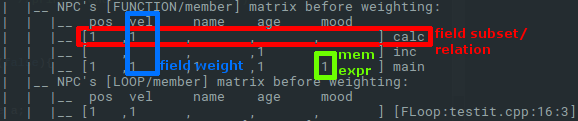
\includegraphics[width=0.7\textwidth, height=0.2\textwidth]{PICs/npc_crosscheck_matrix_relations}
	\caption{Relations depicted in function/member matrices}\label{npc_crosscheck_matrix_relations}
\end{figure}
Fields' relations to each other need to be valued, too. After all their correlation will work best, if they end up as hot data together. The aim is for their temporal locality to result in improved spatial locality. Each group of field usages (function) needs to somehow weight its collective field impact, to heighten their chance to stay together as hot data. We prioritize small groups, since externalizing more fields (with low usage frequency) will result in less stride. Functions will therefore compete against each other, by adding to their field weights the overall number of fields minus the amount of fields they utilize. This scales with the number of fields a record has. As mentioned before instead of brute forcing our way through each possible split combination we now encode each field subset relation numerically so eventually it will influence a field's overall weight. It is important to form a decision over an overall weight because unlike an optimization for a specific algorithm, changing the programs data layout has the potential to affect ALL of its functions.

\subsection{Field weight heuristics}\label{field_weight_heuristics}
When we are able to define a field's overall weight on a program, whats left to do is finding a delimiter, that actually divides the field set in two subsets, depending on those weights. This again is not a trivial operation and first of all we need to define what we intend to separate.\\
As can be seen in the Figures \ref{avg_delimiter} to \ref{avg_delimiter_bad_5} we will face numerous different situations that result of arbitrary access patterns. While sometimes it is easy to rule out certain fields, for others it is not. A generic set of rules to handle this needs to be able to process special cases while not losing credibility for common ones. It can do so by scaling with the problem.
\subsubsection{Scaling delimiters}
Scaling delimiters will adjust automatically as the problem changes. In a lot of cases a very easy heuristic will work comparably well. For example a (we will call it) \textit{max/2} where we will just take the maximum field weight and divide it by two. Everything above the \textit{max/2} will be hot and vice versa. Given our 'scope' is the maximum field weight this will yield very good results for a lot of cases, however the more significant the spikes are, the worse will be the affects on the resulting data layout. While the \textit{max/2} regards quality it dismisses quantitative scaling.\\\\
A surprisingly easy yet effective candidate is the average, because it scales up when certain fields tend to be a lot more important than others and naturally divides our values according to their relative weight \reffigp{avg_delimiter} unlike for example their median value.
\begin{figure}[ht]
	\begin{minipage}[b]{0.5\linewidth}
		\centering
		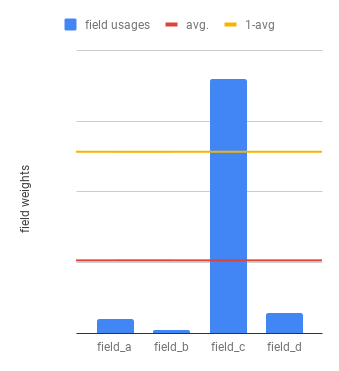
\includegraphics[width=\textwidth,height=.7\textwidth]{PICs/avg_as_delimiter_1}
		\caption{Good avg scaling.}
		\label{avg_delimiter}
	\end{minipage}
	\hspace{0.5cm}
	\begin{minipage}[b]{0.5\linewidth}
		\centering
		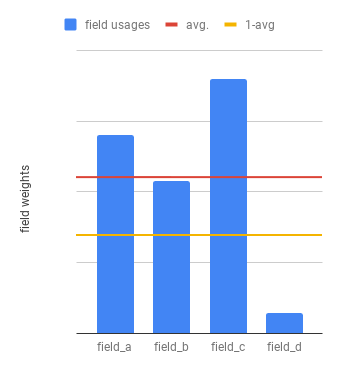
\includegraphics[width=\textwidth,height=.7\textwidth]{PICs/avg_as_delimiter_2}
		\caption{Difficult evaluation for avg scaling.}
		\label{avg_delimiter_bad}
	\end{minipage}
	\hspace{0.5cm}
	\begin{minipage}[b]{0.5\linewidth}
		\centering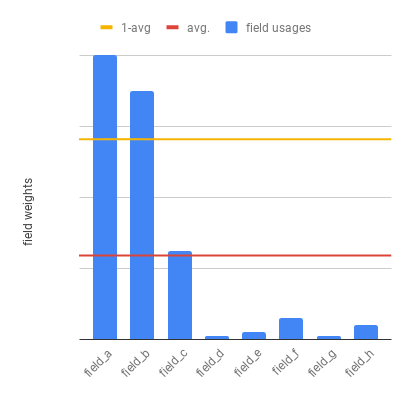
\includegraphics[width=\textwidth,height=0.7\textwidth]{PICs/avg_as_delimiter_3}
		\caption{Bad avg scaling with more fields.}
		\label{avg_delimiter_bad_2}
	\end{minipage}
	\hspace{0.5cm}
	\begin{minipage}[b]{0.5\linewidth}
		\centering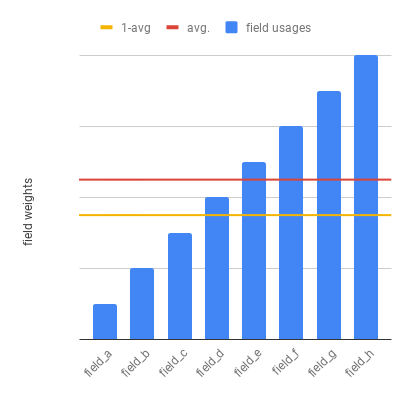
\includegraphics[width=\textwidth,height=0.7\textwidth]{PICs/avg_as_delimiter_4}
		\caption{Problem of even distribution.}
		\label{avg_delimiter_bad_3}
	\end{minipage}
\end{figure}
Unfortunately \reffig{avg_delimiter_bad} shows, why sometimes a simple average determination might not be the best fit. If \textit{field\_a} or \textit{field\_c} were slightly less important, \textit{field\_b} would probably be considered hot, yet this way, even though its rating is far from \textit{impactless} it is considered to be cold.\\
On the other hand \reffig{avg_delimiter_bad_2} shows why an average will also not scale well with the amount of fields in a record. The average narrows as the divisor grows, so on a record with a hand full of members an average might end up introducing fields to the hot subset that barely pass the average weight.\\\\
This leads to an interesting dilemma; where to draw the line between hot and cold fields? Should there be constant \textit{magic numbers} defining the threshold of a hot field? Since different access patterns can produce arbitrary field weightings there is no good way of predicting a constant, that suffices our intention. But how can relative proportions work when they introduce false-positives? And can we get rid of them? \reffig{avg_delimiter_bad_3} illustrates a difficult case that will in practice rarely occur but embodies our problem perfectly. An even distribution of field weights allows for no logical grouping of significance, at least in terms of 'drawing the line'.
\begin{figure}[ht]
	\begin{minipage}[b]{0.5\linewidth}
		\centering
		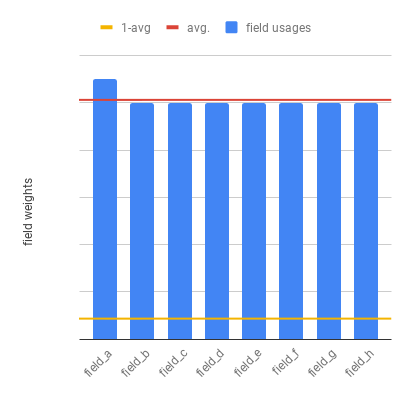
\includegraphics[width=\textwidth,height=.7\textwidth]{PICs/avg_as_delimiter_5}
		\caption{Bad avg homogeneous field weights.}
		\label{avg_delimiter_bad_4}
	\end{minipage}
	\hspace{0.5cm}
	\begin{minipage}[b]{0.5\linewidth}
		\centering
		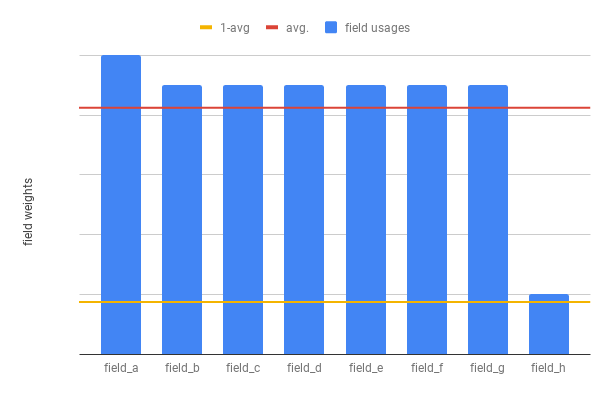
\includegraphics[width=\textwidth,height=.7\textwidth]{PICs/avg_as_delimiter_6}
		\caption{\textit{1-avg} prone to false positives as well.}
		\label{avg_delimiter_bad_5}
	\end{minipage}
\end{figure}
The average as a heuristic fails us in many situations. We referred to it because it provides a quick approximation of a good delimiter. The factors however that determine its scaling are contrary to the paradigms we follow. Number-of-fields as a divisor means decreasing averages with increasing amount of fields. This means the more fields our records have (consequently the more lack of cohesion), the higher the collective chance to be considered hot. Also the average behaves poorly towards well designed records. Consider \reffig{avg_delimiter_bad_4} where \textit{field\_a}'s weight is just slightly higher than the others'. It will deem all fields but \textit{field\_a} cold and probably ruin the data layout.\\\\
The above diagrams propose another heuristic that we will call the \textit{1-avg}, represented by the yellow lines. It introduces the reciprocal counterpart for the averages bad scalings. By taking the greatest field height minus the average, our tolerance for fields grows linearly as the average rises while regarding the overall scope of our field weights. In other words: The more quality we find in a record (the more the average trends towards the maximum field weight) the more fields we allow to be hot.\\
As can be seen in the above figures, this heuristic behaves much better for records that show great differences in their field weights. Of course it is very much possible for it to behave poorly in specific situations as well, again coming from spikes. \reffig{avg_delimiter_bad_5} shows, that the reciprocal average quickly becomes too tolerant. We have seen, that \textit{1-avg} is able to correct some mistakes the average makes but it introduces unwanted behavior on its own.\\

\subsubsection{Combined scaling delimiters}
An interesting take is on how to combine certain scaling delimiters. Depending on the case different heuristics will result in drastic deterioration of the data layout. We could try to avoid such errors by cherry-picking the strengths different heuristics provide.\\
One possibility could be to adapt the \textit{max/2} heuristic. We can determine both the \textit{avg} and the \textit{1-avg} delimiters, take the greater one and divide it by 2 (we will call it \textit{top/2}). The upper delimiter will always separate the most significant fields for us. As the \textit{max/2} easily gave us a quick way of defining a tolerance towards lower significant fields, it did not in any way regard the fields' quantity as a defining factor. By possibly considering the \textit{1-avg} (when it is greater) we adapt it given the right situation. This already yields improved results, is however still prone to special cases \reffigp{top_2}. This is because we do not consider the possibility of the cold remnant to be relevant in its entirety.
\begin{figure}[!ht]
	\begin{minipage}[b]{0.5\linewidth}
		\centering
		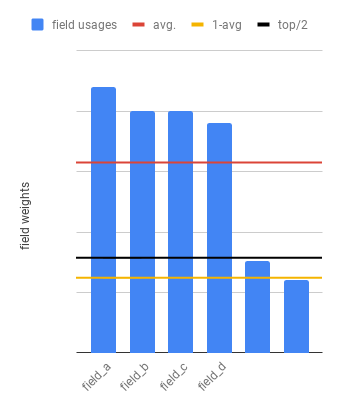
\includegraphics[width=\textwidth,height=.8\textwidth]{PICs/top_2}	
	\end{minipage}
	\hspace{0.5cm}
	\begin{minipage}[b]{0.5\linewidth}
		\centering
		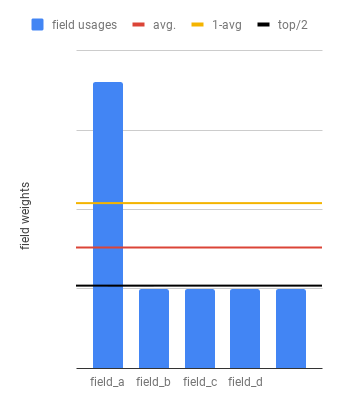
\includegraphics[width=\textwidth,height=.8\textwidth]{PICs/top_2_bad}
	\end{minipage}
	\caption{Improved \textit{top/2} heuristic as it is able to rule out \textit{1-avg} errors but still not well.}\label{top_2}
\end{figure}
The problem with scaling delimiters is, that no matter how much we narrow down the error by applying a certain heuristic, in another distribution the same approach might behave badly in terms of handling another error source. We need to evaluate subsets of fields ordered by significance to reliably rule them out or keep them collectively.\\\\
Regarding both the \textit{avg} and the \textit{1-avg} is interesting because combined they are able to categorize the field weights to a certain extend. As mentioned before, there are two major scaling factors the fields' weights and their number. As the \textit{1-avg} is the reciprocal of the \textit{avg} we can derive information about a programs access patterns by looking whether \textit{avg} or \textit{1-avg} is greater than the other.\\
When the \textit{avg} is greater, the fields' weights is proportionally more significant than the record's number of fields. When the \textit{1-avg} is greater on the other hand, it means that proportionally there are more insignificant fields than the subgroup of 'important/hot' fields. Well designed records will demonstrate $avg\approx f_{max}$. Anyhow we can interpret those two delimiters as an order of significance. They divide our scope into three spaces. One above the greater delimiter, one below the smaller delimiter and whatever is in between them \reffigp{delimiter_tiers}. Fields in the upper space are certainly to be considered hot. Fields below the lower line are in a less significant order. Whatever is in between is what we can not categorize immediately. 
\begin{figure}[!ht]
	\begin{minipage}[b]{0.5\linewidth}
		\centering
		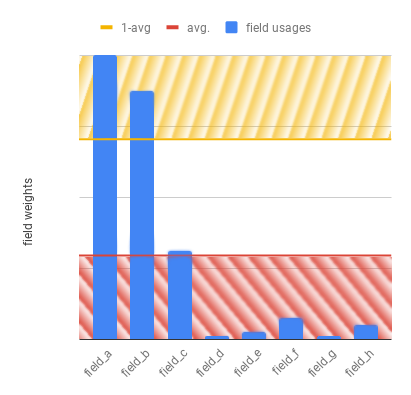
\includegraphics[width=\textwidth,height=.7\textwidth]{PICs/delimiter_tiers}	
	\end{minipage}
	\hspace{0.5cm}
	\begin{minipage}[b]{0.5\linewidth}
		\centering
		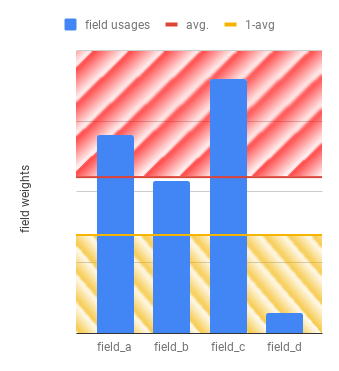
\includegraphics[width=\textwidth,height=.7\textwidth]{PICs/delimiter_tiers_2}
	\end{minipage}
	\caption{Field weight categorization by combined scaling delimiters. Top hatched space is of high significance.}\label{delimiter_tiers}
\end{figure}
The idea is to now recursively apply the ordering between the \textit{avg} and the \textit{1-avg} delimiters as long as we have fields, that we can neither classify as high- nor little significance. This approach will work fine with data sets, that exhibit high significance varieties. On uniformly distributed field weights it will tend to include the whole field set for the hot data, yet since we encoded logical relations in the field weight a distribution like in Figure \ref{avg_delimiter_bad_3} bespeaks of defective access patterns rather than only bad data layout.\\
Regarding order of significance is a good approach to a generic solution, yet our recursive approach is not optimal since it is based on scaling delimiters, that are unaware of a field-group's collective impact. Also trying to break down a record's significance order into two (hot \& cold) subsets immediately mitigates precision.

\subsubsection{Order of significance / Significance groups}\label{sig_groups}
The problem is that until now we tried to divide a record in two subsets, which actually is our intention, but the truth is there can be an arbitrary amount of related subsets in the record's data fields and the more significance groups we have and the greater the difference in significance, the blurrier the delimiter becomes. Delimiters based on either quantitative or qualitative scaling introduce an error of a size we can hardly reason about when compared to the entirety of field weights \reffigp{delimiter_bad}. Percental tolerance factors will also always just move the error resulting in better behavior in some situations and worse in others.\\
Also one of the worst situations for us is to accidentally separate fields, that are logically related. With scaling delimiters it can easily happen, that two fields, that share an order of significance (due to our metric) are separated because the delimiter ever so slightly includes one of them but excludes the other. Whenever we split fields that are codependent we ensure worsened cache utilization, because the functions that use the hot field will most likely also use the cold field and will now have the additional overhead of the indirection to the cold struct instance. Our Recursive approach tried to solve this issue and will succeed in simple cases, yet ultimately it depends on the blurry scaling delimiters.\\\\
Scaling delimiters try to evaluate field weights individually, yet their sub-/optimal utilization strongly depends on their significance group. Determining whether or not a field should be considered hot should depend on the benefit/punishment of its extraction. Externalizing a field always means that the remaining hot fields load less unnecessary stride into a cache-line, yet it also means whenever the extracted field is used, unrelated cold data might be loaded as well.\\
Cache-lines have concrete sizes (e.g. 64 Byte) so at this point we might be tempted to just multiply a field's size in byte to its weight. This way it is possible to see the field's impact on the cache capacity and evaluate whether or not determining a certain field as cold would imply great punishment. On the other hand, this way the least frequently used field could suddenly be considered hot if it is just big enough. We may not confuse capacity with usage frequency, which is the actual criteria of a Hot/Cold Split \refsec{hot_cold_splitting}. So it is actually enough to compare our field weights as a criteria for benefit and punishment. However in order to determine a significance group's impact on our program we are definitely interested in comparing its size to the cache-line size in order to deduce possible stride (which we want to reduce after all).\\\\
But how can we determine significance groups? COOPs approach is to sort the fields according to their weights in a descending order and measure their weight differences. Normalized on the scope ($f_{max}$) we can compare them to the average deviation. Each value above the average will denote a new, less significant group that spans until the next group is identified \reffigp{sig_order}.
\begin{figure}[ht]
	\begin{minipage}[b]{0.5\linewidth}
		\centering
		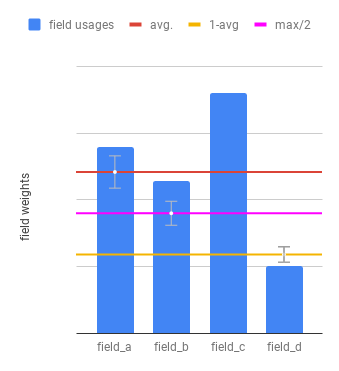
\includegraphics[width=0.8\textwidth,height=.7\textwidth]{PICs/delimiter_bad}
		\caption{Scaling delimiters' errors can hardly be reasoned about and provide equally much punishment as benefit depending on the distribution.}
		\label{delimiter_bad}
	\end{minipage}
	\hspace{0.5cm}
	\begin{minipage}[b]{0.5\linewidth}
		\centering
		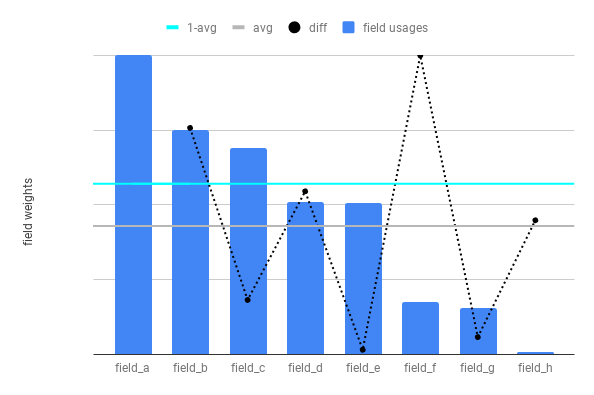
\includegraphics[width=\textwidth,height=.7\textwidth]{PICs/sig_order}
		\caption{Determination of significance groups with field weight deltas. Normalized differences are projected on the field weights' scale for visualization.}
		\label{sig_order}
	\end{minipage}
\end{figure}
The important thing is for the fields to be evaluated in terms of groups rather than individually. To do so it is crucial to know, how to even evaluate a group. First we need to determine the group's benefit/punishment in case of a split. Each significance group $g_i$ has a type size $s_i$ which is the summarized type sizes of its fields, as well as a $max_i$ which is its highest field weight. With the cache-line size $CLS$, the general cold struct indirection overhead $H$ and with $n$ as the amount of significance groups, when a group $g_i$ is extracted, it implies the following:\\
Extracting $g_i$ means $s_i$ less stride for the remaining hot data. We already ordered the fields' weights in a descending order, so now we can compare their type sizes with the additional space and as soon, as one or more of the hot fields fit in the additional space (minus $H$) we will effectively have reduced the number of cache-lines to fit 1 hot data instance by the factor $\frac{s_i}{CLS}$ (without splitting an addressable unit over two cache-lines). So the benefit will express through the re-utilization of the hot fields which is capped to the highest field weight of the hot fields ($F_{max}$ or $max_0$). We can value it by multiplying the $F_{max}$ with the determined benefit. This practically tells us how many cache-lines we will spare our important procedures.\\
But we can make our estimation a little better by interpreting each significance group as a representation for those procedures (loops/functions), that have contributed to it. So instead of capping our 'savings' estimation on the most significant value ($F_{max}$) we will take each significance groups maximal field weight, as this value represents the groups estimated loads. So our savings $s(g)$ are:
\begin{align}
	s(g_i) = \sum_{k=0}^{i-1}max_k\cdot\frac{-H+\sum_{k=i}^{n}s_k}{CLS}
\end{align}
At this point our procedure will cut off everything until the last group of highest significance, because we have not yet determined the 'costs' of externalizing a significance group as a counter weight. As the stride is reduced for the hot subset it is increased in the cold subset. The payoff for a hot set is the additional indirection over the pointer to the cold struct instance. When applied correctly this is however comparably little as we plan to externalize greater means.\\
The cold data will always be accessed by going through the hot data (the pointer to the cold data is in the hot data). So whenever we are accessing cold data we automatically waste one cache-line per cold struct instance that is used to load and dereference the pointer to it. In terms of cache utilization this is unfortunate not only in terms of capacity, but also because of possible thrashing because the hot and cold data lie at physically different locations \refsecp{cpucu}. It is only worth because we do it with data, that is accessed so rarely (relatively), that this cost is lower than the benefit we get by splitting it from the hot data. However, besides the additionally wasted cache-lines used solely for finding the actual data, we will increase the cold data's stride by $s_i$ Byte, resulting in an estimated iteration overhead $o(g)$ of
\begin{align}
	o(g_i) = \sum_{k=i}^{n}max_k\cdot(1+\frac{\sum_{k=i}^{n}s_k}{CLS})
\end{align}
cache-lines for processing the cold data in its entirety. Ultimately for each $g_i$ we say that a split is worth $w(g)$ when:
\begin{align}
	w(g_i) = s(g_i) > o(g_i)
\end{align}
Then we want to externalize it because the estimated benefit is greater than the estimated cost.\\\\
Unfortunately this will only work for tightly packed arrays of data, since we assume, that reduced stride immediately results in improved cache utilization. If we implemented an automatic SOA transformation this would be the way to go \refsecp{soa}. Due to alignment issues \refsecp{memory_management} COOP will allocate the hot and cold data in a way that is not exactly packed, but will consider alignments, so to a certain extend a reduced stride will have virtually no effect other than the additional indirection to the cold data - invalidating our progress so far.\\
To be more specific COOP will regard the target systems L1 D (configurable depending on optimization preferences) cache-line size and will try to pack as many elements into a line, yet align each entity group to the cache-lines, to prevent unnecessarily much entity splits over too many cache-lines  (we briefly discussed this in \refsec{aosoa}). This means, that when our hot subset size is smaller than the target cache-line, reducing the stride will have effect, as soon as it frees enough space for the cache-line to encompass another instance \reffigp{opt_p_1}.\\
On the other hand, if the hot subset size is greater than the cache-line, reduced stride will have effect, as soon as it results in reducing the number of cache-lines necessary to encompass an instance \reffigp{opt_p_2}. So actually since we will introduce padding due to our alignment we might even want to consider keeping poorly ranked fields, as long as they only replace space, that otherwise would be used for padding.
\begin{figure}[ht]
	\begin{minipage}[b]{0.5\linewidth}
		\centering
		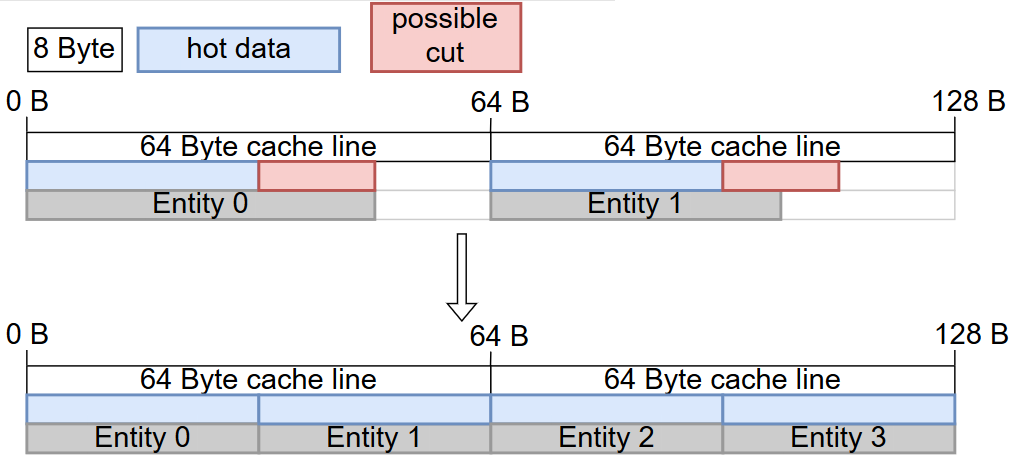
\includegraphics[width=\textwidth,height=.6\textwidth]{PICs/opt_possibility_1}
		\caption{Aligned entities will be packed inside cache-lines. Reduced stride will be effective, as soon as it increases the amount of entities inside a cache-line.}
		\label{opt_p_1}
	\end{minipage}
	\hspace{0.5cm}
	\begin{minipage}[b]{0.5\linewidth}
		\centering
		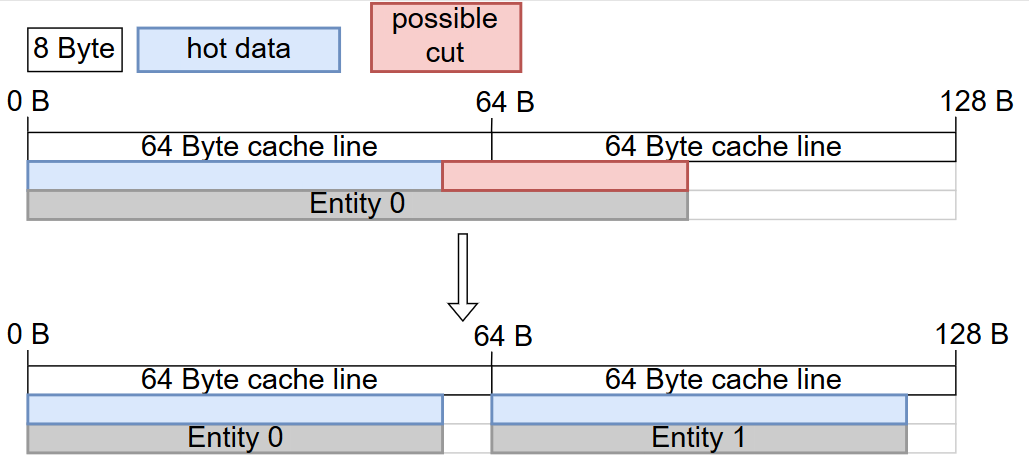
\includegraphics[width=\textwidth,height=.6\textwidth]{PICs/opt_possibility_2}
		\caption{Reduced stride will be effective as soon as it reduces the number of cache-lines needed to encompass an entity. Entities are split upon minimum amount of lines.}
		\label{opt_p_2}
	\end{minipage}
\end{figure}
Again this needs proper evaluation, since at this point our procedure will blindly cut out fields because it can not reason about the splits impact to its full extent. We again need to include our field weights into the equation, to be able to evaluate whether or not a split will result in more benefit, than punishment.
More formally for a significance group $g_i$ our heuristic $W(g)$ will consider a split beneficial when:
\begin{equation*}
W(g_i) =
\begin{cases}
\scalemath{1.2}{\myceil{\frac{CLS}{\sum_{k=0}^{i-1}s_k}}} > \scalemath{1.2}{\myceil{\frac{CLS}{\sum_{k=0}^{i}s_k}}} \land w(g_i) & \text{for}\sum_{k=0}^{n}s_k < CLS\\\\
\scalemath{1.2}{\myceil{\frac{\sum_{k=0}^{i-1}s_k}{CLS}}} < \scalemath{1.2}{\myceil{\frac{\sum_{k=0}^{i}s_k}{CLS}}} \land w(g_i) & \text{for}\sum_{k=0}^{n}s_k > CLS
\end{cases}
\end{equation*}
It is worth to note here, that this consideration of the groups type sizes is another kind of scaling that we have not had considered before. This heuristic will yield different results depending on the actual type sizes and will therefore be more precise in its evaluation. Scaling delimiters solely relying on comparing the field weights will tend to split over aggressively, because they do not consider that the benefit of a split depends also on how the resulted record's will interact with a specific target cache. In fact, to actually accomplish an improvement, a cut will now need to extend a certain threshold. So in many cases COOP will now rather do nothing, than trying to force a split, that will actually worsen the cache utilization.\\\\
\begin{figure}[tbp]
	\centering
	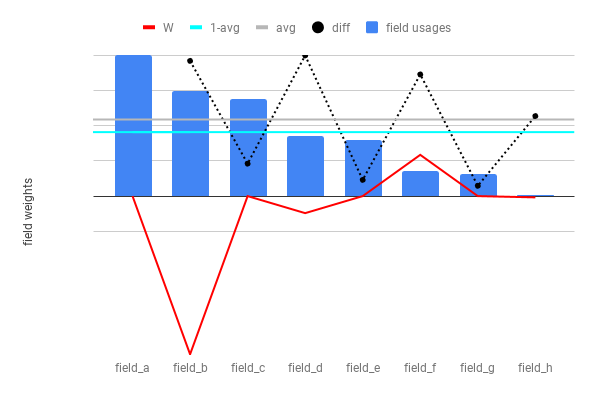
\includegraphics[width=0.8\textwidth,height=0.5\textwidth]{PICs/sig_order_final}
	\caption{Exemplary field weights evaluated by our heuristic with the result, that its worth to make the split hot:[\textit{field\_a}, ...\textit{field\_e}], cold:[\textit{field\_d}, ...\textit{field\_h}].}
	\label{sig_order_final}
\end{figure}
Unfortunately this heuristic might be problematic, as soon as we deal with significant spikes. Imagine a field, that outweighs the others. Since we only consider significance groups as split candidates (opposed to fields individually) we will now compare $n-1$ fields to be split. This might actually make sense, because the highly rated single field might provide well enough cache utilization to outweigh the externalization of the rest, however we will strip ourselves from optimization potential as soon, as deviation significance leads to false positives on field to group assignment. When the significance group that field is assigned to, is not considered to be worthy of externalizing, but individually the falsely assigned field would be, we produced an error. Assigning a field to a significance group, that in reality should be in a lower order group, will prevent this field from being examined distinctively. So again we are limited by scaling delimiters, only this time when evaluating delta deviation instead of quality. Even though this is a special case, it is not unlikely enough to be disregarded.\\\\
One possible solution is to again follow a recursive approach. Whenever significance groups are identified we can recursively apply the procedure inside the distinct groups to identify more groups, but without a fitting recursion break, this will eventually lead to creating $n$ groups for $n$ fields.\\
It is hard to reason about when to stop the recursion, because forth going each group will have its own significance scope and therefore will evaluate its internal discrepancies differently - relatively more significant. To a certain extend this is exactly what we want, but at the same time it will eventually lead to over-grouping. What we need is an atomic unit that denotes a step of significance. This way instead of losing the scope in recursion, we will have a recursion-depth independent measure.

\subsubsection{A brief discourse to data analysis in statistics}
The methodology defined in statistics can yield very good results for our intention, however statistics are usually applied to large sets of data. A record with a number of fields that validates it to be examined statistically will rarely (if ever) be found in practice, however the methodology can be applied to our problem partially.\\\\
We could improve the significance groups' granularity and their robustness by applying measurements, that are known to behave better with spikes in their \textit{population} or that can help us detect such spikes, so we can adapt our routines. Norbert Henze describes different \textit{measures of dispersion} \mcp{henze}{32}, that we can consider. Statistically significant spikes can for example be identified by determining the \textit{empiric standard deviation} for a population. The standard deviation (usually denoted as $\sigma$) is defined as:
\begin{align}
\scalemath{1.2}{\sigma} := +\sqrt{\frac{1}{n} \sum \limits_{i=1}^n\left(x_i-\overline x\right)^2}
\end{align}
It can be used to quantize the order of discrepancy to the norm. If a value for example is $2\sigma$ it is more likely to be significant, $3\sigma$ even more so. Consequently we could define that as soon as a field weight delta $f_i-f_{i-1}>T\sigma$ (where $f$ is a field weight and $T$ is an arbitrary constant) we would need a distinct significance grouping starting from $f_i$, since including  field weights prior to $i$ could compromise the significance group assignment for low ordered field weights.\\\\
Another measure of classification is the \textit{interquartile range} (IQR). It describes the difference between the upper- and the lower most quartiles and is mostly resistant to spikes, because it operates on the median instead of the arithmetic mean. Significant discrepancies can be determined by orders of IQR units. For a set of elements $x = (x_1, x_2, ..., x_n)$ that is ordered, the IQR is defined by the difference of the upper and lower quartiles $x_{0.25}$ and $x_{0,75}$ which are the respective medians of the elements to the left and right of the median $\tilde{x}$.
\begin{align}
x_{0{,}25} = \begin{cases}
\tfrac{1}{2}(x_{n \cdot 0{,}25} + x_{(n \cdot 0{,}25) + 1}),  & \text{if }n \text{ is even}\\
x_{\lfloor n \cdot 0{,}25 +1\rfloor}, & \text{if }n \text{ is odd}
\end{cases}\\
x_{0{,}75} = \begin{cases}
\tfrac{1}{2}(x_{n \cdot 0{,}75} + x_{(n \cdot 0{,}75) + 1}),  & \text{if }n \text{ is even}\\
x_{\lfloor n \cdot 0{,}75 +1\rfloor}, & \text{if }n \text{ is odd}
\end{cases}
\end{align}
The IQR which is then determined by subtracting $x_{0,75}-x_{0,25}$ describes for us the range of the 50\% of the elements around the median $\tilde{x}$. However this does not mean that each value above $\tilde{x}+\frac{1}{2}\cdot IQR$ is considered a significant spike.\\
A famous practical application of the IQR are \textit{Box-Plot}s \mcp{boxplot}{916} which are a popular utensil for quickly describing data distributions and possible spikes. They define spikes to be $> T\cdot IQR$, where $T$ is a constant that is often between four and seven. However pin-pointing those 'spike thresholds' usually depends on the populations environment.\\
We could apply this methodology to identify spikes in the field weight deltas so we could determine which ranges (expressed in quartiles) need their own significance grouping. Also identifying fields with weightings below the defined low spike level could immediately associated as cold fields, as we can guarantee, that at least 75\% of the other fields are more significant.\\\\
The methods above rely on constants, that are determined by experience and plausibility. Our algorithm can not yet rely on statistically relevant data to define those constants, yet we are able to make a plausible assumption. The higher we define the threshold for a spike to be, the more tolerant we are for inaccuracies on the other end respectively. The closer we define our thresholds to $x_{0,25}$ and $x_{0,74}$ the higher the chance, that we identify local maxima/minima as spikes, which will lead to similar problems as blurry scaling delimiters (separating fields, that belong together).\\
Since the IQR defines the 50\% of elements around the median, this range also defines a bound of significance. In theory $0,5\cdot IQR+IQR+0,5\cdot IQR$ should define the whole range of elements if they share an order of significance. In order to prevent local maxima/minima to be identified as spikes we will tweak this assumption to $3\cdot IQR$. This will identify spikes relatively quickly and induce a more fine granular significance ordering.

\section{COOP's affect on the data layout}\label{affect_on_data_layout}
Until now we have seen how COOP is able to make an educated guess about the logic relations (expressed in temporal locality) and the computational impact of a field. Even though static analysis will rarely be able to predict a programs data flow precisely (because of run-time dependent variables) we have developed a way that combines traits coming from different metrics to hint at what fields might be the most relevant to us. The numbers (for example access frequencies) will in reality diverge from those we have assumed, however we have succeeded when our educated guess resembles the proportions of run-time data.\\\\
Even though we have set up the basis for a successful split at this point COOP's results would be surprisingly bad/mediocre, depending on the tested target code. Until now we have identified fields to be hot or cold and are able to separate them accordingly. We are affecting the fields' layouts inside their record, but have not yet considered how the records are laid out in memory.\\
The whole point of the AOS to SOA/HotColdSplit/Component/AOSOA transformations we discussed in \refsec{dod} is to improve spatial locality of our data. The actual benefit is the result of reduced stride and a better instance-size to cache-line-size ratio. By identifying temporal locality of our data, we can infer, that spatial locality on those data will result in better cache utilization. But at this point the instances of the record we are examining might be allocated on the heap completely scattered. With scattered heap segments like that, reduced stride in our records will have no effect, since subsequent segments of the memory (expected by the common access patterns we discussed in \refsec{cdap}) will most likely be unrelated to our 'hot' data. Cache prefetching mechanisms will not be able to accommodate us. We can never expect to find a successor instance inside an already loaded cache-line.\\ 
In this scenario we will even have separated the 'cold' data and therefore taken what little correlation the hot and the cold data had. So depending on how the data is distributed in memory until now our optimization might behave good, but just as well might deteriorate the cache utilization.\\\\
Another important part is the allocation of the cold data. By our definition fields are separated when the remaining hot data benefits from the split more, than the cold data suffers from it. By this definition it might very well happen that we extrude fields, that are used comparably little, but this does not mean, that those fields are used infrequently in their routines. Only because a \textit{field\_a} was assigned a field weight of e.g. $720,000$ the extracted cold field \textit{field\_d} with a field weight of $35,000$ can not be regarded impact-less. We deemed it beneficial to split \textit{field\_d}, but that does not mean we shall ignore it.\\
Cold fields might just as well participate in routines that abide the access patterns, we can optimize around. For example a particles position and velocity might very likely be considered hot, the particle's field \textit{radius} will also be used frequently, but our heuristic recognized it to be little enough to warrant a split. The routines that use radius will most likely do so for a bunch of particles in a row. Making sure the cold data is packed in contiguous blocks of memory will improve those 'cold' routines.\\
Consequently COOP will not only parse the target program for instance allocations, that tend to behave badly, but also care about the cold structs to be allocated in a cache friendly manner.

\subsection{Hot data allocations we want to adapt}\label{hdawwta}
There are different ways to obtain memory to hold data. Specifically when executing a C++ program the compiler will have made precautions to reserve memory for e.g. the actual code, variables known at compile time, a block of memory to hold local variables \mcp{stroustrup}{587}.\\
We are especially interested in the data segments \textit{stack}, \textit{heap}, as well as \textit{.bss} \textit{.data}, because this is where the target program will reserve memory of the records we aim to split. Static and global variables exist in the \textit{.data} segment (when initialized) and the \textit{.bss} (if uninitialized). Local variables are placed on the stack. An instance that is allocated with e.g. \textit{malloc, calloc} or \textit{new} is placed on the \textit{heap}. Note for later: the \textit{.bss} will not actually affect the object file's size. The loader will merely zero initialize it (also depends on the OS) on program start \mcp{bryant}{659}.\\\\
We want our data to be in contiguous memory blocks. With techniques like \textit{placement new} we can easily transform the target code to place data where we want it but we should also clarify what specific allocations we want and can change without hurting cache utilization or corrupting semantic integrity. So whenever we find a statement, that allocates memory for a record that we want to split, we can change it in a way that will hopefully leave the succeeding code unaffected \refcodep{alloc_changes}.
\begin{lstlisting}[language=C++,name={Examples of how we can change allocations using placement new to emplace the data where it is among related data.},label={alloc_changes}]
Foo all_foos[N];

//Foo f_0;   becomes:
all_foos[i] = Foo();
Foo &f_0 = all_foos[i]; //NOT OK: semantic integrity corrupted
...
//Foo f_1[10];   becomes:
Foo *f_1 = new (all_foos+i) Foo[10]; //NOT OK: semantic integrity corrupted
...
//Foo *f_2 = new Foo();   becomes:
Foo *f_2 = new (all_foos+i) Foo();  //OK: conserved semantic integrity
...
//Foo *f_3 = new Foo[10];   becomes:
Foo *f_3 = new (all_foos+i) Foo[10];  //OK: conserved semantic integrity
\end{lstlisting}
However these changes imply using some index \textit{i} that will determine the data's new location in the Foo collection \textit{all\_foos}. More importantly while a local variables lifetime is bound to it's scope, now it 'lives' in the \textit{all\_foos} and we will manually need to clean it up properly when we reached the variables original deadline, as well as maintaining the index \textit{i} so it will again provide \textit{all\_foos+i} as allocatable memory. For the placement new variant there should exist a respective \textit{delete} call that we will need to change as well. Instead of the delete call we will want to invoke that instance's destructor manually and manage the memory address on our own.\\
However local variables are intended to live and work inside the scope they are defined in. In terms of cache utilization we should assume, that their creation implies temporal locality with all the other local variables of that same scope so at this point we probably should not try to force it to live among data, that it will not share contextual relation with.\\
Also we can not maintain semantic integrity when changing local variables. We have effectively changed the data types of \textit{f\_0} and \textit{f\_1} which will break successive statements easily or just cause subtle bugs (consider how \textit{sizeof} will still work, but yield different results for \textit{f\_0} and \textit{f\_1}). Maintaining semantic integrity can only work, when working with pointer types.\\
In case of \textit{f\_3} the target program already does handle its data in data structures, that suffice the intention of contiguous memory blocks. Without further static analysis we can not predict which data allocation might have been intended regarding principles of locality. If an array allocation like this happens more than once in a program, these distinct blocks of memory might still correlate, but they might just as well be 'bundled' because they constitute one logic unit of computation. Forcing them to exist among other instances of their kind will most likely not provide additional benefit and as stated before without further static analysis we can not properly reason about them. To avoid breaking the code unnecessarily or to disturb a data flow that we deem optimal anyway, we only want to 'correct' the instance allocations, that lead to scattered related data. In other words: single instance heap allocations of hot data.\\
There is a specific initialization pattern, we target and that is high frequent heap accesses. Whenever we want to set up an array of pointers for a record we will probably engage a loop that iterates the pointers, calling new a lot. For each time the new operator is invoked we will undergo a context switch into kernel mode search a memory block of appropriate size in the heap context switch back into user mode \mcp{gregory}{427}. Depending on the heaps fragmentation this will scatter the instances all over our free memory. What we want instead is for those instances to be emplaced in some predefined contiguous block of memory.

\subsection{Customized memory management for split records / COOP's free list}\label{memory_management}
A contiguous block of memory for our hot data instances will prevent them from laying across the programs free memory. This way minimized stride will result in improved cache utilization. However the moment we initialize instances in our own predefined scope of memory we need to manage that space on our own. This is what custom allocators are used for.
However assuming that block-wise initialization of data in the target source code is done intentionally, we do not want to interfere with it. Instead we will focus on providing management utensils to prevent high frequent heap access, as discussed in the previous section \refsecp{hdawwta}. There are many different implementations of custom allocators, but usually they are used to either allocate fixed sized blocks of memory or provide a demanded capacity dynamically. Since we will only handle single instance allocation COOP's custom memory management system will somewhat be a special case of a \textit{fixed block allocator} where the block size is the records size. In other words what we want is a so called \textit{pool allocator} \mcp{gregory}{430}.\\
COOP will inject a data structure into the target project, that is able to find and free available space without adding significant run-time overhead. A rather simple implementation for our pool allocator is a \textit{Free List}.\\\\
But first of all we need to inject code into the target source code, that will reserve us some memory. The data we will want to manage with our free list would have originally lived in the free memory. The heap can make use of the entire addressable space which exceeds the stack. So we do not want to move all those data to the stack, because this would potentially overflow quickly, depending on how extensively the target source code allocates heap memory. We could also rely on dynamic allocations, however in order to minimize manual memory management obligations we will instead target a static data segment. COOP will ultimately inject (templated!) code into the target project, so in order to keep the resulting object files' sizes minimal we will use the \textit{.bss} segment. The \textit{.bss} section occupies no actual space, the object file merely needs to remember how much space it will have to demand on program load \mcp{bryant}{659}. On Unix systems the \textit{size} command line tool is a handy utensil for investigating this. For example when creating a simple \textit{bss.cpp} file with an uninitialized global array of 3 \textit{int}s and another \textit{data.cpp} file with an initialized array of 3 \textit{int}s we can investigate their object files' segment sizes, as well as their file sizes like this: \reffigp{seg_sizes}
\begin{figure}[!htbp]
	\centering
	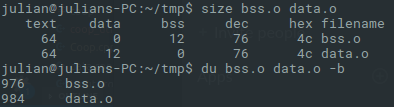
\includegraphics[width=0.5\textwidth, height=0.2\textwidth]{PICs/bss_data_comparison}
	\caption{Comparison of .bss and .data sizes for different initializations.}
	\label{seg_sizes}
\end{figure}
\begin{lstlisting}[language=C++,name={Code injection to generate contiguous block of memory for a record Foo's instances.},morekeywords={constexpr, size_t, coop_free_list},label={cont_mem_foo}]
constexpr size_t hot_size_plus_ali_NPC =
	coop::size_plus_alignments(N, alignment, element_size);

constexpr size_t cold_size_plus_ali_NPC =
	coop::size_plus_alignments(M, alignment, element_size);

char byte_data_Foo[hot_size_plus_ali_Foo + cold_size_plus_ali_Foo];

coop_free_list hot_free_list_instance_Foo(
	byte_data_Foo,
	byte_data_Foo+hot_size_plus_ali_Foo,
	alignment, sizeof(Foo));

coop_free_list cold_free_list_instance_Foo(
	byte_data_Foo+hot_size_plus_ali_Foo,
	byte_data_Foo+hot_size_plus_ali_Foo+cold_size_plus_ali_Foo,
	alignment, sizeof(coop_cold_fields_Foo));
\end{lstlisting}
So for a split record \textit{Foo}, COOP will generate code injections like in \refcode{cont_mem_foo} in order to reserve the appropriate amount of contiguous memory space. Line 1 to 5 in \refcode{cont_mem_foo} determine how much memory in Byte we need to encompass all instances. In line seven we reserve the actual memory (uninitialized \textit{.bss}) which will be the combined sizes of the hot and the cold data for the record Foo. In line 9 to 17 we create the free list instances. \refcode{cont_mem_foo} also shows that we rely on some additional variables and computations here. The sizes of the memory block, that our free lists will manage, need to be adjusted to the way the free list will operate. As mentioned before in \refsec{field_weight_heuristics} to maximize access efficiency we will align our data. On the one hand we will pack as much instances together in a cache-line, on the other hand we will align those instance groups to the cache-lines alignment. This way we will possibly generate some padding between those instance groups, but we also guarantee, that the minimum amount of cache-lines is needed to load an instance. Disadvantageous strides will not lead to instances being separated among more cache-lines than necessary.\\
But now whenever this results in additional bytes for padding, we also effectively increased the necessary memory space to encompass all our entities. This is what the \textit{size\_plus\_alignments(size\_t number\_elements, size\_t alignment, size\_t element\_size)} function does. It takes the number of entities \textit{N} we expect during run time (line 2), the \textit{alignment} that we will need to adjust on, and the \textit{element\_size} which will for example be the size of our record Foo.\\
The padding per instance group is dependent on whether or not the record's size is equal to, greater than or smaller than the cache-line size and defined like this (where \textit{S} is the record's size in Byte and \textit{CLS} the cache-line size):
\begin{align}
pad\_per\_group = \begin{cases}
	 0\text{ for } S == CLS\\
	(\myfloor{\frac{S}{CLS}} +1)\cdot CLS - S \text{ for } S > CLS\\
	CLS - (\myfloor{\frac{CLS}{S}}\cdot S) \text{ for } S < CLS
\end{cases}
\end{align} \\\\
The element size is also not just \textit{sizeof(Foo)}, because we need to consider the possibility for a very small record to be split. For example if record Foo consisted of only an int (4 Byte) and a long int (8 Byte) and we wanted to split the long int away, leaving us with a single 4 Byte. As we will see when we explore the free list, it depends on its entities to be at least the size of a pointer, so it can properly resemble a linked list. That's why the \textit{element\_size} will be the maximum of the size in Byte of Foo and a Foo pointer type, to guarantee the free list to work as intended.\\
When we have the padding per instance group we can calculate how much capacity we need to encompass all our elements including their groups' padding respectively (where \textit{m} is the number of instances per group, \textit{n} is the total amount of instances):
\begin{align}
	capacity = (m\cdot S + pad\_per\_group)\cdot \myceil{\frac{n}{m}}+CLS
\end{align}
The alignment is the target cache's alignment, which COOP will retrieve from the system on program start. On Unix systems information on the caches can be found in \textit{sys/devices/system/cpu/cpu}<CPU ID>\textit{/cache/index}<cache ID>. For example the file \textit{sys/devices/.../type} contains whether or not this cache is a data cache or not. The file \textit{coherency\_line\_size} will contain the cache-line size in Byte.\\
The same is done for the record Foo's new cold field struct. But the number of elements ratio between the record and its cold struct pendant will (should) not be 1:1 for reasons we will discuss in \refsec{deep_copy_emulation}. For now its left to say, that \textit{N} and \textit{M} will be determined by the user, as we can not predict how many instances will actually be made.\\\\
Finally the free list instances are created (\refcode{cont_mem_foo} line 9 to 14) which will be given the byte range they will administer, as well as the target cache's line size and the 'chunk' size (which is just our record's size).
\begin{lstlisting}[language=C++,name={Shortened excerpt of COOP's free list without asserts and some initialization code.},morekeywords={constexpr, size_t},label={free_list}]
	class coop_free_list	{
	...
	coop_fre_list(char *data_start, char *data_end, size_t alignment, size_t block_size){
		...
		for(size_t Ts = 0; free_ptr < end; free_ptr = *next)
		{
			if(++Ts > Ts_per_chunk)
			Ts = 1;
			
			*next =
				free_ptr+block_size+(Ts == Ts_per_chunk ? padding_to_next : 0);
			
			if(*next >= end){*next = nullptr; break;}
		}
		free_ptr = begin;
	}
	
	template<typename T> T * get()
	{
		T *ret = union_cast<T*>(free_ptr);
		free_ptr = *next;
		return ret;
	}
	
	void free(void *p)
	{
		char *tmp_ptr = free_ptr;
		free_ptr = union_cast<char*>(p);
		*next = tmp_ptr;
	}
private:
	union {
		char *free_ptr;
		char **next;
	};
	char * begin = nullptr;
	char * end = nullptr;
	};
\end{lstlisting}
The \textit{coop\_free\_list} itself will only have three fields. Two char pointers (\textit{begin} and \textit{end}) which will mainly be used for bounds checking and a union containing a char pointer \textit{free\_ptr} that can also be used as a pointer to a char pointer.\\
In their essence free lists are only linked lists. Linked lists usually contain several nodes, that are linked to their successors, sometimes their predecessors and depending on specific implementations even more pointers to relevant nodes like the list head and end. I classic introductions to linked lists, nodes are allocated dynamically and a linked list can therefore grow (and spread) over the free memory. A linked list's nodes usually contain a data element, that in our case would hold the concrete instance and one or more pointers to other nodes,so the list can be iterated by following the trail the pointers constitute. In the case of a free list we want to work with contiguous memory blocks instead. Also to further work towards beneficial cache behavior it utilizes the data's memory space to also contain the pointer information to other 'nodes'. Each respective memory range, that will encompass an instance, will actually contain the pointer to the next element, whenever it does not at the moment represent an existing instance \reffigp{free_list_in_memory}.\\
Since we especially want to handle single instance allocations and pack those into cache-line groups we will need further effort to ensure that those groups are aligned optimally. \refcode{free_list}'s lines 3 to 15 contain an important part of the free lists constructor. Here we initially iterate over our entire range to set up the adjacency relations of our 'nodes'. Until this point we already determined the number of instances per cache-line group (or chunk). The free list instance will work with any data type, but will almost entirely work with char pointers to avoid unnecessary much templated code. However since 'generic' data types are often represented as \textit{T}, the number of instances per chunk will here be \textit{Ts\_per\_chunk}.\\
Starting at an address, that will initially be aligned to a cache-line we will treat it as a pointer to a char pointer instead of a char pointer, so we can emplace the information of where to find the next node in it (line 7 to 13). This is a simple operation, because we know the size of an instance (our \textit{block\_size}). Since the block size encodes Byte units we can just add it to the address of this iteration to get the address of the upcoming element. Doing so we will count towards the \textit{Ts\_per\_chunk}. When we exceed the number of elements in a cache-line group, instead of only adding the block\_size to the current address we will also add the necessary padding we determined earlier to jump towards the next aligned address and start a new cache-line group \reffigp{free_list_in_memory}.\\
Treating the current address as a pointer to a char pointer is possible by accessing it through the union's \textit{char **next}. 
\begin{figure}[!htbp]
	\centering
	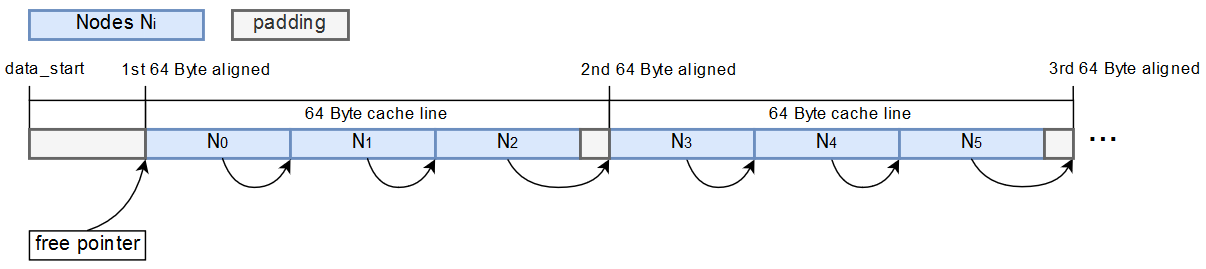
\includegraphics[width=0.86\textwidth, height=0.3\textwidth]{PICs/free_list_in_memory}
	\caption{The free list's layout in memory. Starting with a (possible) initial padding, the instances here represented by nodes will be grouped in a way, that a maximum amount of nodes fits a cache-line. Each group is again aligned to the cache-lines (here 64 Byte) to guarantee minimal loads.}
	\label{free_list_in_memory}
\end{figure}
To obtain a pointer to an element the free list provides the \textit{get} method which will simply return the actual free pointer and declare the 'next' node to be the currently free element (\refcode{free_list} line 18 to 23). It is equally easy to declare an instance's node as free space again, by caching the current free pointer in a temporary variable, setting the actual free pointer to the newly free address and declaring it's 'next' element as the cached variable (\refcode{free_list} line 25 to 30).

\subsubsection{Problematic fragmentation}
Just like the free memory ultimately our free list is prone to fragmentation, as soon, as the target program's instances 'die' more frequently as well as randomly. On the one hand we do not have to worry about a for loop trying to iterate over all the elements in the free list, by merely iterating an index variable over the original array, because our free list is injected into the code and therefore the target code will have no interaction with our free list other than the ones we intend to. But fragmentation still hurts us, as it will deteriorate the number of instances to cache-lines ratio. For example when we have three instances in a cache-line group and 'destroy' every first and second element our instance : cache-line ratio will effectively have gone from 3:1 to 1:1.\\\\
However as new elements are created the 'holes' in between the actual data blocks will refill. Pool allocators are inherently robust when it comes to fragmentation. So In certain situations, where our target program requires a lot of instances, deletes a random subset of them regressing our instance to cache-line ratio to 1:1, we might encounter non optimal cache utilization.\\\\
This is a special case and might be neglected but a possible solution would be for our free list's to shift blocks of memory together. More specifically whenever an address is freed, we could take the last element and place it there. This way no matter how the \textit{get}/\textit{free} ratio of the target program would be, our data instances would be contiguous in memory. But it is not that easy. Since we actually shifted the data, a pointer to that data is now invalid.\\
To sustain the pointer it could either be a smart pointer, that observes the free list, reacting to changes, or our pool allocator could provide a second array solely consisting of pointers, to the original data array. The \textit{get} method would now return an index to the pointer array and the corresponding pointer would lead to the actual data. Whenever data is shifted the pointer array is traversed and updated accordingly. Whoever is holding an index to the pointer array, will now access the actual data through an additional indirection \mcp{gregory}{440}.\\
This could solve the fragmentation for special data lifetime patterns, but as mentioned above pool allocators are themselves quite robust to fragmentation so at this point its worth mentioning in case the pool allocator proves to be unqualified provide improved cache-utilization on its own.\\\\
Beneficial alignments of quasi continuous entity groups in memory can strongly affect a target programs cache utilization. With our heuristic considering the field's type sizes in Byte and the target cache's line-size we are moving away from making an educated guess towards calculating actual relations between a split and it's cache utilization. Measurements will show, that this approach is improving decision making on splits, however we are going to notice, that sometimes but not always our formulas are off a bit. Not meaning there is some sort of race condition going on. It rather depends on the project we are testing. To be more specific, it depends on the record declarations we are examining and the record sizes of the resulting split records. It might happen, that a target programs hot-record size is different from what we calculated when we tried to make a decision whether or not a split at a certain point is beneficial or not. Why this might be the case is going to be explained in the following.

\subsection{Structure Padding and field reordering}\label{structure_padding_and_field_reordering}
\begin{wrapfigure}[10]{r}{0.35\textwidth}
\vspace{-1cm}
\begin{lstlisting}[language=C++,numbers=none,name={Example field declarations to elaborate on structure padding},label={padding}]
char c;//+3B (possibly)
int i;

struct Foo{
	float f1;//+4B padding
	int *i_ptr;
	float f2;//+4B padding
};
\end{lstlisting}
\end{wrapfigure}
Whenever we work with fields of data, in C++ we do so by associating a type declaration to it. A field's type on first glance is nothing but a piece of information on how much actual space we need to reserve in memory to suffice our data's capacity. For \refcode{padding}'s char definition \textit{c} and int \textit{i} we could assume, that their layout in memory resembles their definitions in the source code, meaning there is one Byte for the char \textit{c} and the following next four Bytes are reserved for our int \textit{i}. Now sometimes and arguably most of the times this assumption will be valid, however depending on the particular address of \textit{c} in memory \textit{c}'s immediate succeeding Bytes will not belong to \textit{i}.\\\\
For our modern processors compilers lay out memory abiding alignment constraints in order to make accessing them faster \mc{padding}. We already talked about how COOP will align its data managed by the free list, so that an instance will be split upon a minimal amount of cache-lines. In the best case this means finding an instance's data on one cache-line entirely. This is done, so we can guarantee a minimal amount of main memory loads, when accessing our data. As we learned those main memory loads can be very expensive so aligning data in a way that reduces load operations can have a significant impact on run time performance.\\
This is also what compilers do, when generating machine code for our field declarations. Accordingly, any data type has a defined alignment requirement, that is the information on how to align this piece of memory to guarantee optimal access performance. While chars encompass only a single Byte, they can be placed anywhere without further alignment requirements. Four Byte floats, or ints for example must be placed at an address divisible by four; Eight Byte longs or doubles at addresses divisible by eight and so on. This is sometimes referred to as them being \textit{self-aligned}. One can manually arrange for the compiler to ignore alignment requirements (e.g. using pragma pack, or invoking the compiler with certain command line parameters), however this virtually always comes with punishment in terms of performance, so it is advised not to do so, unless its unavoidable \mc{padding}.\\
Not aligning a data type not only implicates unnecessary many loads, but also results in additional effort for the memory controller, since in order to operate on the data it must now mask, shift and logically OR the two together into a CPU register, so the imminent operations can treat it normally \mcp{gregory}{160}.\\\\
Let us get back to our example \refcode{padding}. In order to abide alignment requirements, depending on where char \textit{c} lays in memory, our char \textit{i} might follow a three Byte long hole of padding. The same goes for field declarations inside record definitions. While the float \textit{Foo::f1} is guaranteed to abide its alignment requirement (we will shortly see why) the int pointer \textit{Foo::i\_ptr} will need to follow a four Byte padding in order to be aligned correctly. Float \textit{f2} follows a higher alignment requirement, which suffices its own requirements (All alignment requirements are powers of two).\\
The compiler will add one last padding to this record definition, because it considers the possibility of struct \textit{Foo} to be used in continuous blocks of memory. In order not to invalidate the field paddings we need to ensure, that they are correct for each successional instance. This can be done by aligning the record to its highest field alignment requirement. For our struct \textit{Foo} this means, that in order to suffice the eight Byte alignment requirement we need trailing padding of an additional four Byte. Consequently the size of our struct \textit{Foo} is not 16, but 24 Byte. Defining \textit{Foo}'s fields in a different order could get rid of (in this case) unnecessary padding but essentially this explains how on certain test files COOP's methodology to determine a favorable split will not match the actual situation.\\
When considering a split for a certain subset of fields, there is not yet an actual compiled version of it. We do not have the means to call \textit{sizeof(non-existent-record)} on it, so either we implement a JIT compiler to momentarily compile a version of our record, or we consider structure padding ourselves. Merely summarizing the field's type sizes will not be enough, as it may disregard possible structure padding.\\
In \refsec{sig_groups} we defined our formula on how to determine whether or not a split at a certain point is favorable or not. In order for this formula to work properly it needs to consider a theoretical split-record's structure padding.\\
We have seen, that records can be defined in suboptimal ways. We also came to the conclusion before in \refsec{rtasl} that padding just like unused data is effectively lost potential in terms of cache utilization and we also have the means to 'improve' the target definitions layout. COOP will in fact rearrange a record's field definitions in a descending order (descending alignment requirements) to avoid unnecessary structure padding. With this COOP is able to get rid of most padding Bytes.\\\\
In \refsec{scirl} some major problems that this approach implicates are going to be discussed. Actually this topic really hints at why an optimization like this can \textbf{never} be considered 'legal' or safe in terms of C++ language compliance and we will see, why COOP will work fine in some situations but in principal can not work.




